\chapter{Requirement Engineering}
This chapter describes the requirement engineering process, including requirements elicitation, analysis, and specification. The goal of this process was to identify and define the requirements that would guide the design of the system.


\section{Requirements Elicitation}
During the requirement elicitation phase, functional and non-functional requirements were identified through an initial brainstorming session, informed by the authors' domain knowledge in robotics. This was complemented by a review of relevant literature and existing work to extract common requirements and established best practices for comparable systems (see Chapter \ref{chapter:related-work}). The process was iterative, with requirements continuously refined as the understanding of the problem domain and potential solution space evolved. This resulted in an initial set of requirements that informed the subsequent requirement analysis.

It is acknowledged that the absence of direct input from end-users and stakeholders introduces limitations. In particular, misalignment between system functionality and user needs may lead to reduced usability and thus increased development effort due to rework of the system. Incorporating stakeholder feedback during the requirements phase, through methods such as interviews, surveys, or workshops, would help mitigate these risks and likely improve the overall quality of the system.


\section{Requirements Analysis}
\subsection{Use Cases}
To further refine and structure the system requirements, use cases were employed. Use cases provide a scenario-based perspective of system functionality by describing how actors interact with the system to achieve specific goals. This approach complements the previously identified requirements. The development of the use cases followed a systematic process described below.

First, the relevant actors were identified. Actors represent entities that interact with the system, either as users or as external systems. In this project, two primary actors were defined: the Developer, representing the end-user interacting directly with the system, and the LLM Provider, representing the external service supplying large language model capabilities. The FERA vector database was also considered as an actor, but it was ultimately not included as the database is not part of this project as described in the scope (see Section \ref{sec:introduction:scope}).

\begin{table}[H]
    \centering
    \begin{tabular}{p{2.5cm}p{11.5cm}}
        \toprule
        \textbf{Actor} & \textbf{Description}                                                                                       \\
        \midrule
        Developer      & A user who interacts with the system to search, understand, and edit robotic programs.                     \\
        LLM Provider   & An external service that provides large language model capabilities to support the system's functionality. \\
        \bottomrule
    \end{tabular}
    \caption{List of actors.}
    \label{tab:requirement-engineering:actors}
\end{table}

\vspace{-0.1cm}
Next, the use cases were identified. These correspond to the main functionalities the system must support. For the Developer, the primary use cases include searching, editing, uploading, and exporting robot programs. In addition, the system provides LLM-assisted functionality through the use case "Get LLM assisted support". This captures interactions where the system leverages the LLM to assist the user. This high-level LLM-assisted use case was further refined into more specific functionalities, namely: answering user questions, generating robot programs, modifying existing programs, and debugging robot programs. These represent distinct goals that can be achieved through the LLM integration. A validate/simulate robot program use case was also considered, but ultimately not included as it goes beyond the scope of this project.

\begin{table}[H]
    \centering
    \begin{tabular}{p{4cm}p{10cm}}
        \toprule
        \textbf{Use Case}        & \textbf{Description}                                                                                                                                     \\
        \midrule
        Search robot programs    & The Developer can search for relevant robotic programs based on natural language queries.                                                                \\
        Edit robot program       & The Developer can edit existing robotic programs to adapt them to new contexts.                                                                          \\
        Upload robot program     & The Developer can upload their own robotic programs to edit using the system and for inclusion in the repositories and identification in future queries. \\
        Export robot program     & The Developer can export robotic programs from the system.                                                                                               \\
        Get LLM assisted support & The Developer can receive assistance from the LLM to support various tasks related to robotic program development.                                       \\
        Answer user questions    & The system can answer user questions related to robotic programs and documentation using the LLM.                                                        \\
        Generate robot program   & The system can generate new robotic programs based on user input using the LLM.                                                                          \\
        Modify existing program  & The system can modify existing robotic programs based on user input using the LLM.                                                                       \\
        Debug robot program      & The system can assist in debugging robotic programs by identifying potential issues and suggesting fixes using the LLM.                                  \\
        \bottomrule
    \end{tabular}
    \caption{List of use cases.}
    \label{tab:requirement-engineering:use-cases}
\end{table}

\vspace{-0.1cm}
Following this, associations between actors and use cases were established. The Developer is connected to all primary use cases, reflecting direct interaction with the system's features. The LLM Provider is associated with the LLM-assisted support functionalities, indicating that these capabilities depend on an external service.

A system boundary was then defined to clearly distinguish between the internal system functionality and external actors. All use cases are contained within this boundary, while the actors remain outside, interacting with the system through defined interfaces.

Finally, relationships between use cases were modeled. The "Get LLM assisted support" use case is represented as an extension of the "Edit robot program" use case, indicating that assistance is an optional feature that can enhance the editing process. Additionally, the more specific LLM-related use cases can be seen as generalizations of the assistance functionality, providing more detailed descriptions of how the system supports the user.

\subsection{Use Case Diagram}
The resulting use case diagram is shown in Figure \ref{fig:requirement-engineering:use-case-diagram}. It provides an overview of the system's functionality, the involved actors, and the relationships between different interactions. This diagram contributes to refining the initial requirements by clarifying system functionality and interactions, and serves as a foundation for the subsequent system design.

\begin{figure}[H]
    \centering
    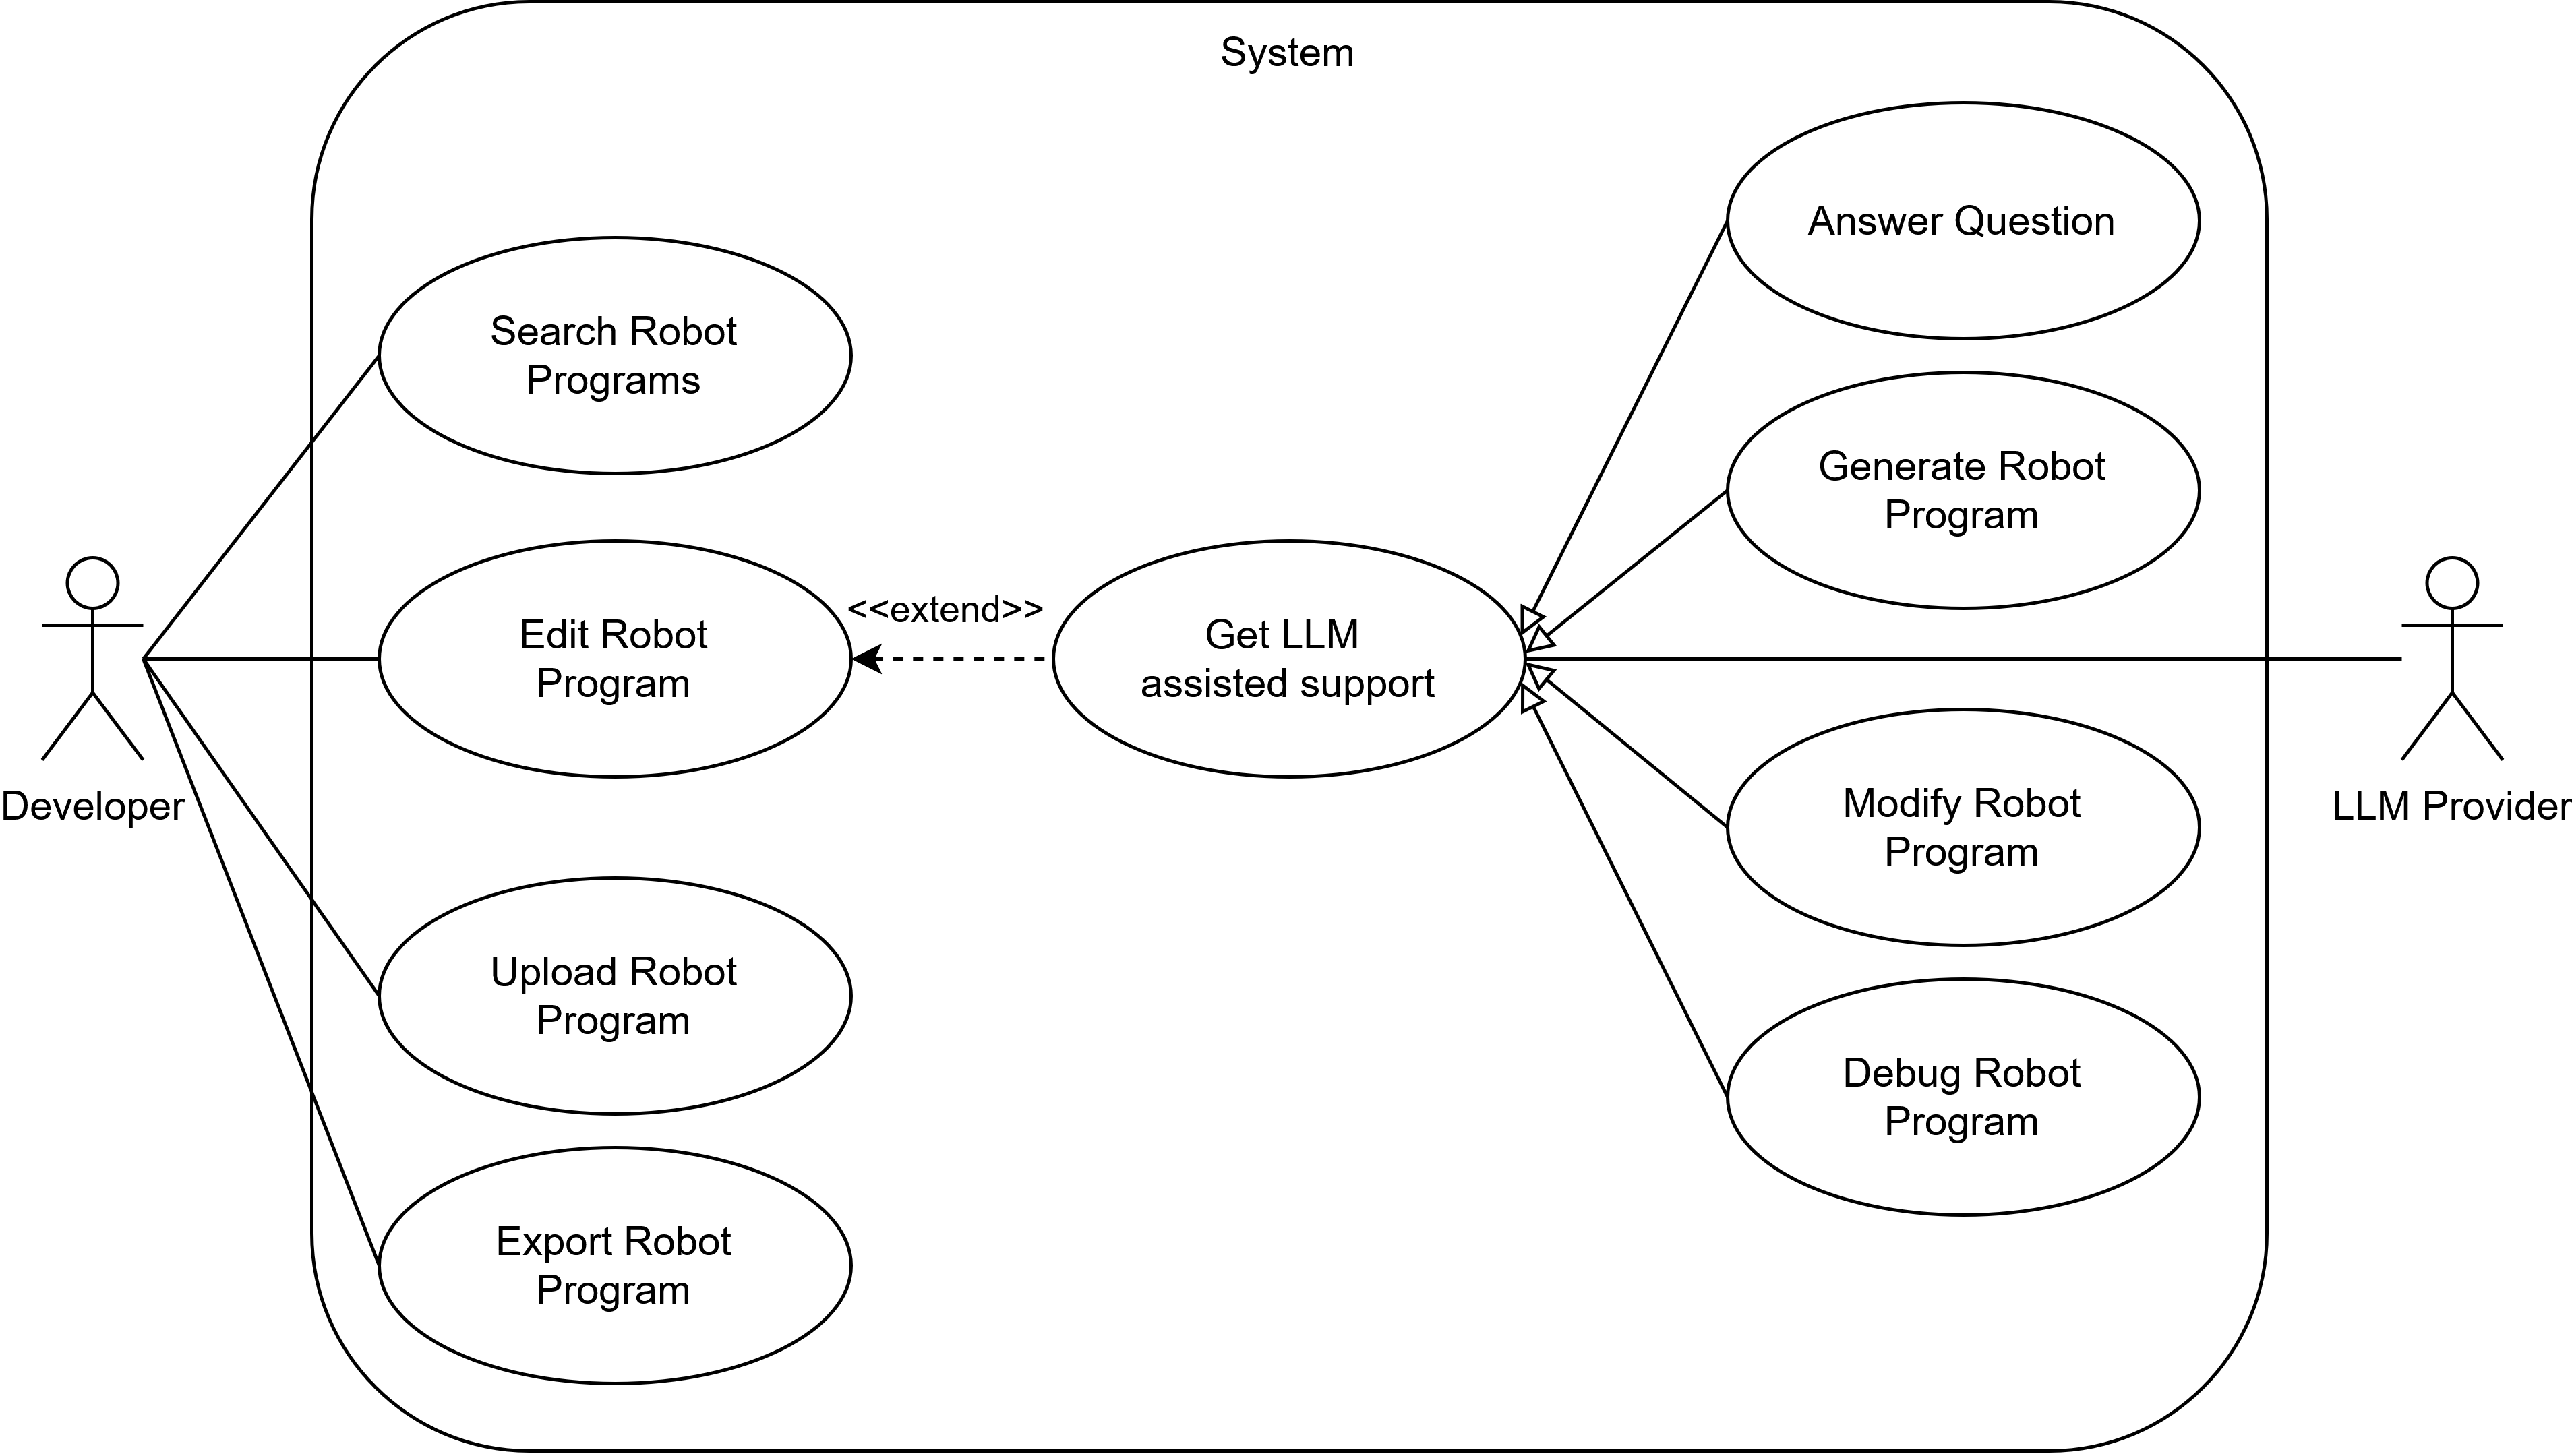
\includegraphics[width=\columnwidth]{media/use-case-diagram.png}
    \caption{{Use Case Diagram.}}
    \label{fig:requirement-engineering:use-case-diagram}
\end{figure}


\section{Requirements Specification} \label{sec:requirement_engineering:specification}
The final set of functional and non-functional requirements is specified below.

\textbf{Functional Requirements (FR):}
\begin{adjustwidth}{\indentWidthTwenty}{\indentWidthTwenty}
    \textit{\textbf{System:}}
\end{adjustwidth}
\begin{adjustwidth}{\indentWidthForty}{\indentWidthForty}
    \textit{\textbf{FR1:} The system shall allow searching for robot programs to identify programs for future development.}
\end{adjustwidth}
\begin{adjustwidth}{\indentWidthForty}{\indentWidthForty}
    \textit{\textbf{FR2:} The system shall allow for uploading robotic programs for inclusion in the program repository and identification in future queries.}
\end{adjustwidth}
\begin{adjustwidth}{\indentWidthForty}{\indentWidthForty}
    \textit{\textbf{FR3:} The system shall allow for exporting robot programs.}
\end{adjustwidth}
\begin{adjustwidth}{\indentWidthForty}{\indentWidthForty}
    \textit{\textbf{FR4:} The system shall provide a robot program editor.}
\end{adjustwidth}
\begin{adjustwidth}{\indentWidthForty}{\indentWidthForty}
    \textit{\textbf{FR5:} The system shall provide LLM-assisted support by answering user queries expressed in natural language.}
\end{adjustwidth}

\begin{adjustwidth}{\indentWidthTwenty}{\indentWidthTwenty}
    \textit{\textbf{AI Assistant:}}
\end{adjustwidth}
\begin{adjustwidth}{\indentWidthForty}{\indentWidthForty}
    \textit{\textbf{FR6:} The AI assistant responses shall be human-readable.}
\end{adjustwidth}
\begin{adjustwidth}{\indentWidthForty}{\indentWidthForty}
    \textit{\textbf{FR7:} The AI assistant shall support the user in comprehending robotic programs by answering user questions.}
\end{adjustwidth}
\begin{adjustwidth}{\indentWidthForty}{\indentWidthForty}
    \textit{\textbf{FR8:} The AI assistant shall support modification tasks by suggesting changes to existing robot programs based on user instructions.}
\end{adjustwidth}
\begin{adjustwidth}{\indentWidthForty}{\indentWidthForty}
    \textit{\textbf{FR9:} The AI assistant shall retain relevant conversational context within a session to support follow-up questions.}
\end{adjustwidth}
\begin{adjustwidth}{\indentWidthForty}{\indentWidthForty}
    \textit{\textbf{FR10:} The AI assistant shall indicate uncertainty when the available information is insufficient to provide a reliable answer.}
\end{adjustwidth}


\textbf{Non-Functional Requirements (NFR):}
\begin{adjustwidth}{\indentWidthTwenty}{\indentWidthTwenty}
    \textit{\textbf{Performance:}}
\end{adjustwidth}
\begin{adjustwidth}{\indentWidthForty}{\indentWidthForty}
    \textit{\textbf{NFR1:} The system shall provide responses to user queries within 10 seconds.}
\end{adjustwidth}

\begin{adjustwidth}{\indentWidthTwenty}{\indentWidthTwenty}
    \textbf{Modifiability:}
\end{adjustwidth}
\begin{adjustwidth}{\indentWidthForty}{\indentWidthForty}
    \textit{\textbf{NFR2:} LLM-specific functionality shall be isolated from core system components to enable integration of alternative language models with minimal implementation effort.}
\end{adjustwidth}

\begin{adjustwidth}{\indentWidthTwenty}{\indentWidthTwenty}
    \textbf{Observability:}
\end{adjustwidth}
\begin{adjustwidth}{\indentWidthForty}{\indentWidthForty}
    \textit{\textbf{NFR3:} The system shall log all LLM interactions, including user inputs, generated outputs, timestamps, and request identifiers, to support monitoring, debugging, and traceability.}
\end{adjustwidth}

\begin{adjustwidth}{\indentWidthTwenty}{\indentWidthTwenty}
    \textbf{Traceability:}
\end{adjustwidth}
\begin{adjustwidth}{\indentWidthForty}{\indentWidthForty}
    \textit{\textbf{NFR4:} For all responses generated using retrieval-augmented generation (RAG), the system shall expose the references of the retrieved source documents used during response generation.}
\end{adjustwidth}

\begin{adjustwidth}{\indentWidthTwenty}{\indentWidthTwenty}
    \textit{\textbf{Usability:}}
\end{adjustwidth}
\begin{adjustwidth}{\indentWidthForty}{\indentWidthForty}
    \textit{\textbf{NFR5:} A majority of users shall rate the LLM-supported responses as clear and understandable.}
\end{adjustwidth}
\begin{adjustwidth}{\indentWidthForty}{\indentWidthForty}
    \textit{\textbf{NFR6:} A majority of users shall rate the system as useful for comprehending robotic programs.}
\end{adjustwidth}
\begin{adjustwidth}{\indentWidthForty}{\indentWidthForty}
    \textit{\textbf{NFR7:} A majority of users shall rate the system as useful for modifying robotic programs.}
\end{adjustwidth}
\begin{adjustwidth}{\indentWidthForty}{\indentWidthForty}
    \textit{\textbf{NFR8:} A majority of users shall rate the LLM-supported responses as relevant to the user query.}
\end{adjustwidth}
\begin{adjustwidth}{\indentWidthForty}{\indentWidthForty}
    \textit{\textbf{NFR9:} A majority of users shall rate the LLM-supported responses as factually correct.}
\end{adjustwidth}